\setcounter{subsection}{22-1}
\subsection{The Quotient Topology}

% Useful macros for this section
\def\ivp{\inv{p}}
\newcommand\ivpss[1]{\ivp\parens{\braces{#1}}}
\def\zset{\braces{0}}

\exercise{1}{
  Check the details of Example~3.
}
\sol{
  Recall that Example~22.3 includes a function $p: \reals \to A$ where $A = \braces{a,b,c}$ is a three-point set.
  The function is defined by
  \gath{
    p(x) = \begin{cases}
      a & x > 0 \\
      b & x < 0 \\
      c & x = 0 \,.
    \end{cases}
  }
  We are then asked to verify that the quotient topology on $A$ induced by $p$ is that indicated by the following diagram:
  \begin{center}
    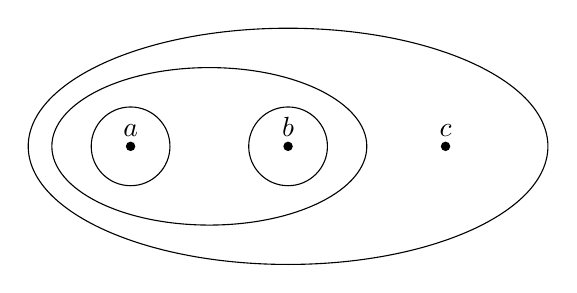
\begin{tikzpicture}
      % Points
      \fill (-2,0) circle (0.06);
      \fill (0,0) circle (0.06);
      \fill (2,0) circle (0.06);

      % Point labels
      \node [above] at (-2,0) {$a$};
      \node [above] at (0,0) {$b$};
      \node [above] at (2,0) {$c$};

      % Single point subsets
      \draw (-2,0) circle (0.5);
      \draw (0,0) circle (0.5);

      % Two-point subsets and full set
      \draw (-1, 0) circle (2 and 1);
      \draw (0, 0) circle (3.3 and 1.5);
    \end{tikzpicture}
  \end{center}
  \qproof{
    Clearly the diagram illustrates the topology $\cT = \braces{\es, \braces{a}, \braces{b}, \braces{a,b}, A}$ on $A$.
    We also note that $p$ is surjective, and that $\cT$ is the unique topology such that $p$ is a quotient map.
    First, obviously $\es$ and $A$ must be open in the quotient topology $\cT$ since it is a topology.
    Then, clearly the following sets
    \ali{
      \ivpss{a} &= (0, \infty) \\
      \ivpss{b} &= (-\infty, 0) \\
      \ivpss{a,b} &= (0, \infty) \cup (-\infty, 0)
    }
    are all open in $\reals$ so that $\braces{a}$, $\braces{b}$, and $\braces{a,b}$ should be open in the quotient topology since $p$ is a quotient map.
    On the contrary, the sets
    \ali{
      \ivpss{c} &= \zset \\
      \ivpss{a,c} &= \clop{0, \infty} \\
      \ivpss{b,c} &= \opcl{-\infty, 0}
    }
    are all clearly not open in $\reals$ (in fact they are all closed) so that $\braces{c}$, $\braces{a,c}$ and $\braces{b,c}$ should not be open in the quotient topology.
    As we have considered all eight of the possible subsets of $A$, this shows the desired result.
  }
}

\exercise{2}{
  \eparts{
  \item Let $p: X \to Y$ be a continuous map.
    Show that if there is a continuous map $f: Y \to X$ such that $p \circ f$ equals the identity map of $Y$, then $p$ is a quotient map.
  \item If $A \ss X$, a \boldit{retraction} of $X$ onto $A$ is a continuous map $r: X \to A$ such that $r(a) = a$ for each $a \in A$.
    Show that a retraction is a quotient map.
  }
}
\sol{
  (a)
  \qproof{
    First, $f$ is a right inverse for $p$ by definition so that $p$ is surjective by Exercise~2.5 part (a).
    Suppose that $U$ is a subset of $Y$.
    If $U$ is open in $Y$ then $\ivp(U)$ is open in $X$ since $p$ is continuous.
    So suppose that $V = \ivp(U)$ is open in $X$.
    Since we have $p \circ f = i_Y$ is bijective and $i_Y = \inv{i_Y}$, it follows from Exercise~2.4 part~(a) that
    \gath{
      U = i_Y(U) = \inv{i_Y}(U) = \inv{(p \circ f)}(U) = \ivf(\ivp(U)) = \ivf(V) \,.
    }
    Then, since $V$ is open in $X$, we have that $\ivf(V) = U$ is open in $Y$ since $f$ is continuous.
    This shows that $p$ is a quotient map by definition.
  }

  (b)
  \qproof{
    Suppose $X$ is a topological space, $A \ss X$, and $r: X \to A$ is a retraction.
    Let $f: A \to X$ be defined by $f(a) = a$ for all $a \in A$, i.e. $f$ is the identity function on $A$ with the range expanded to $X$.
    Now, $i_A$ is continuous (in fact it is a homeomorphism) by Exercise~18.3 so that $f$ is also continuous by Theorem~18.2 part~(e) since it is just $i_A$ with an expanded range.
    Then for any $a \in A$ we have that
    \gath{
      (p \circ f)(a) = p(f(a)) = p(a) = a
    }
    since $p$ is a retraction.
    Thus $p \circ f = i_A$, which shows that $p$ is a quotient map by what was shown in part~(a).
  }
}

\def\realss{\reals \times \reals}
\exercise{3}{
  Let $\pi_1: \realss \to \reals$ be projection on the first coordinate.
  Let $A$ be the subspace of $\realss$ consisting of all points $x \times y$ for which either $x \geq 0$ or $y = 0$ (or both); let $q: A \to \reals$ be obtained by restricting $\pi_1$.
  Show that $q$ is a quotient map that is neither open nor closed.
}
\sol{
  \qproof{
    An illustration of the subspace $A \ss \realss$ is shown below:
    \begin{center}
      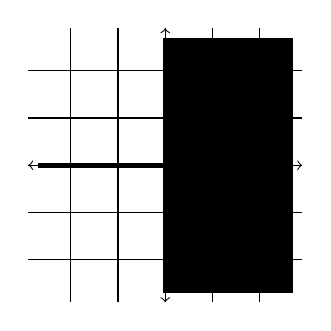
\begin{tikzpicture}[scale=0.6]
        % Fill region
        \fill[fill=black, fill opacity=\tikzgrayopac] (0,-2.7) rectangle (2.7,2.7);

        % Coordinate grid
        \draw[step=1cm,\tikzgridclr,thin] (-2.9,-2.9) grid (2.9,2.9);

        % Axes
        \draw[dashed, <->] (-2.9,0) -- (2.9,0);
        \draw[dashed, <->] (0,-2.9) -- (0,2.9);

        % Boundaries
        \draw[line width=0.6mm] (-2.7,0) -- (0,0);
        \draw[line width=0.6mm] (0,-2.7) -- (0,2.7);

      \end{tikzpicture}
    \end{center}
    First, we know that $\pi_1$ is continuous from \S 18.
    It then follows that the restriction $q$ is a continuous map as well by Theorem~18.2 part~(d).

    Now define a map $f: \reals \to A$ by $f(x) = x \times 0$ for any $x \in \reals$, noting that clearly $f(x) \in A$.
    We show that $f$ is continuous by considering any basis element $U \times V$ of $\realss$ so that $U$ and $V$ are open in $\reals$.
    Now, if either of $U$ or $V$ are empty, then of course $U \times V$ is empty as well so that $\ivf(U \times V) = \ivf(\es) = \es$ is open in $\reals$.
    Otherwise if $0 \notin V$ then also $\ivf(U \times V) = \es$ is open in $\reals$.
    If $0 \in V$ then we claim that $\ivf(U \times V) = U$, which is of course open in $\reals$.
    This is easy to show:
    \ali{
      x \in \ivf(U \times V) &\bic f(x) \in U \times V \\
      &\bic x \times 0 \in U \times V \\
      &\bic x \in U
    }
    since we know that $0 \in V$.
    Thus in all cases $\ivf(U \times V)$ is open in $\reals$, which suffices to show that $f$ is continuous.

    Now consider any $x \in \reals$ so that we have
    \gath{
      (q \circ f)(x) = q(f(x)) = q(x \times 0) = \pi_1(x \times 0) = x \,,
    }
    which shows that $q \circ f = i_\reals$.
    Since $q: A \to \reals$ and $f: \reals \to A$ have both been shown to be continuous, it follows from Exercise~22.1 part~(a) that $q$ is a quotient map as desired.

    To show that $q$ is not an open map, consider that subset $U = \clop{0, 1} \times (1,2) \ss A$, which is open in the subspace $A$ since $U = A \cap [(-1,1) \times (1,2)]$ and clearly $(-1,1) \times (1,2)$ is a basis element of $\realss$ and so is open.
    However, clearly the set $q(U) = \pi_1(U) = \clop{0,1}$ is not open in $\reals$.
    To show that $q$ is not a closed map, consider the set $C = \braces{x \times (1/x) \where x > 0}$.
    It is easy to see and not difficult to show that $C$ is a closed subset of the subspace $A$ because no point of $A - C$ is a limit point of $C$.
    Also clearly $q(C) = \pi_1(C) = \preals$, which is not closed in $\reals$ since its complement $\braces{x \where x \leq 0}$ is not open.
    Thus $q$ is not a closed map either.
  }
}

\newcommand\peqa[1]{x_{#1} + y_{#1}^2}
\newcommand\peqb[1]{x_{#1}^2 + y_{#1}^2}
\newcommand\pptz[1]{#1 \times 0}
\exercise{4}{
  \eparts{
  \item Define an equivalence relation on the plane $X = \reals^2$ as follows:
    \gath{
      \pptt{0} \sim \pptt{1} \condgap \text{if $\peqa{0} = \peqa{1}$.}
    }
    Let $X^*$ be the corresponding quotient space.
    It is homeomorphic to a familiar space; what is it?
    [Hint: Set $g(\pptt{}) = \peqa{}$.]
  \item Repeat (a) for the equivalence relation
    \gath{
      \pptt{0} \sim \pptt{1} \condgap \text{if $\peqb{0} = \peqb{1}$.}
    }
  }
}
\sol{
  (a)
  Two points in the plane are in the same equivalence class if $\peqa{}$ have the same value, say $c$.
  Then we have that $\peqa{} = c$ and hence $x = c - y^2$, which is the equation for horizontally-oriented parabola opening to the left and shifted in $x$ by $c$.
  A few of these parabolic equivalence classes are shown below for various values of $c$:
  \begin{center}
    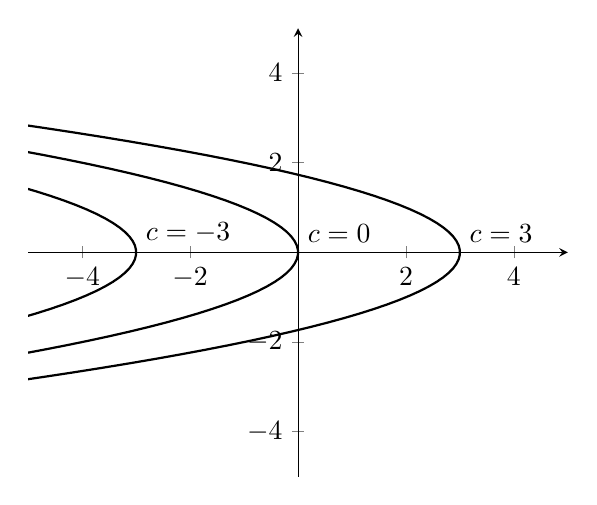
\begin{tikzpicture}
      \begin{axis}[
          axis lines=middle,
          xmin=-5, xmax=5,
          ymin=-5, ymax=5,
          samples=100,
        ]
        \newcommand\parab[1]{
          \addplot[
            black,
            thick,
            domain=-5:5,
          ]
          (#1 - x^2, x);
          \node [above right] at (axis cs:#1,0) {$c=#1$};
        }
        \parab{-3}
        \parab{0}
        \parab{3}
      \end{axis}
    \end{tikzpicture}
  \end{center}
  Then, if $X^*$ is the quotient space induced, by this equivalence relation, then each element of $X^*$ is one of these equivalence classes.
  We claim that this space is homeomorphic to $\reals$.
  \qproof{
    So define $f: X^* \to \reals$ as follows: if $U$ is an equivalence class (so that $U \in X^*$) containing $\pptt{}$ then set $f(U) = \peqa{}$, noting that clearly $f(U) \in \reals$.
    We also note that if $\pptt{0}$ and $\pptt{1}$ are both in the equivalence class $X$ then $\peqa{0} = \peqa{1}$ so that $f(X) = \peqa{0} = \peqa{1}$ is well defined.

    Now suppose that $U_0$ and $U_1$ are two distinct equivalence classes and that $\pptt{0} \in U_0$ and $\pptt{1} \in U_1$.
    It then follows that it is not true that $\pptt{0} \sim \pptt{1}$ so that $\peqa{0} \neq \peqa{1}$.
    Thus we have $f(U_0) = \peqa{0} \neq \peqa{1} = f(U_1)$, which shows that $f$ is injective.
    Next consider any real $c$ and, the point $\pptz{c}$ in the plane, and let $U$ be the equivalence class containing $\pptz{c}$, which must exist since the equivalence classes form a partition of the plane.
    Then we have $f(U) = c + 0^2 = c$, which shows that $f$ is surjective since $c$ was arbitrary.
    This completes the proof that $f$ is a bijection, noting that of course this means that $\ivf$ is also a bijective function.

    Now, the standard topology of $\reals$ of course can have different bases, but we will concern ourselves with the order topology basis first.
    So consider any basis element $B = (a,b)$ of $\reals$ in the order topology.
    Clearly then the inverse image of $B$ is the collection $\cU$ of equivalence classes $U$ where $a < f(U) < b$.
    Then the union of all the sets in $\cU$ is the set of points in the plane $\pptt{}$ where $a < \peqa{} < b$.
    An illustration of such a subset of the plane is illustrated below for $a = -2$ and $b = 3$:
    \begin{center}
      \begin{tikzpicture}
        \begin{axis}[
            axis lines=middle,
            xmin=-5, xmax=5,
            ymin=-5, ymax=5,
            samples=100,
          ]
          \newcommand\parab[2]{
            \addplot[
              name path=#2,
              black,
              thick,
              dashed,
              domain=-5:5,
            ]
            (#1 - x^2, x);
          }
          \parab{-2}{a}
          \parab{3}{b}
          \addplot[
            fill=black,
            fill opacity=\tikzgrayopac,
          ]
          fill between[
            of=a and b,
          ];
        \end{axis}
      \end{tikzpicture}
    \end{center}
    It is easy to see that such a set is open in $\reals^2$ for any $a$ and $b$, which we shall not show formally.
    Thus $\cU$ is an open subset of $X^*$, which suffices to show that $f$ is continuous.

    Now, to show that $\ivf$ is continuous we utilize metric topology bases for both $\reals^2$ and $\reals$, which we know induce the standard topologies on those sets.
    In particular, we use the standard metric $d$ on $\reals$ but use the square metric $\r$ on $\reals^2$, which induces the standard topology on $\reals^2$ by Theorem~20.3.
    Recall that the square metric is defined by
    \gath{
      \r(\pptt{0}, \pptt{1}) = \max\braces{\abs{x_0-x_1}, \abs{y_0-y_1}} \,.
    }
    So consider any $x \in \reals$, let $U$ be the equivalence class in $X^*$ such that $U = \ivf(x)$ so that $f(U) = x$, and let $\cU$ be a neighborhood of $U = \ivf(x)$ in the quotient topology on $X^*$.
    Then we have that $\cU$ is a collection of equivalence classes and that $\pptz{x}$ must be in $U$ since $x + 0^2 = x = f(U)$.
    Clearly also the union $A = \bigcup_{U' \in \cU} U'$ is then open in $\reals^2$ since $\cU$ is open in the quotient space, and $\pptz{x} \in A$ since $\pptz{x} \in U$ and $U \in \cU$.
    Thus by Lemma~\ref{lem:metric:ball} there is a $\d > 0$ where $B_\r(\pptz{x}, \d) \ss A$.

    Now, consider the set $B_d(x, \d)$, which is clearly a neighborhood of $x$ in $\reals$.
    Consider any $V \in \ivf(B_d(x, \d))$ and let $v = f(V)$ so that it must be that $\pptz{v} \in V$ since $v + 0^2 = v = f(V)$.
    Then $v = f(V) \in B_d(x, \d)$ so that $d(v,x) = \abs{v-x} < \d$.
    Since we have $\abs{v-x} \geq 0 = \abs{0-0}$, it follows that
    \gath{
      \r(\pptz{v}, \pptz{x}) = \max\braces{\abs{v-x}, \abs{0-0}} = \abs{v-x} < \d \,,
    }
    and hence $\pptz{v} \in B_\r(\pptz{x}, \d) \ss A = \bigcup_{U' \in \cU} U'$.
    Therefore there is an equivalence class $W$ in $\cU$ such that $\pptz{v} \in W$ and $W \in \cU$.
    However, since the equivalence classes are all disjoint, it has to be that $W = V$ since $\pptz{v} \in V$ as well.
    Thus $V = W \in \cU$ so that $\ivf(B_d(x,\d)) \ss \cU$ since $V$ was arbitrary.
    This suffices to show that $\ivf$ is continuous by Theorem~18.1 since $\cU$ was an arbitrary neighborhood of $U = \ivf(x)$.
    This completes the proof that $f$ is a homeomorphism so that $X^*$ is homeomorphic to $\reals$ as desired.
  }

  (b)
  Here two points are in the same equivalence class if $\peqb{}$ have the same value, say $c$.
  Then we have that the equivalence class is all the points in the plane such that $\peqb{} = c$, which is clearly a circle in the plane with radius $\sqrt{c}$ centered at the origin, noting that of course always $c = \peqb{} \geq 0$.
  We also note that the only point such that $\peqb{} = 0$ is $\pptz{0}$ itself, so this the only point in its equivalence class.
  We claim that the quotient topology on the set of equivalence classes $X^*$ is homeomorphic to the subspace topology of nonnegative reals, i.e. the subspace $A = \braces{x \in \reals \where x \geq 0}$ of $\reals$.
  \qproof{
    Taking a similar approach to that in part~(a), define $f: X^* \to A$ by $f(U) = \norm{\pptt{}} = \sqrt{\peqb{}}$ if $\pptt{}$ is a point in the equivalence class $U$.
    Clearly we have $f(U) \geq 0$ so that $f(U) \in A$.
    It also follows that $f$ is well-defined since, if $\pptt{0}$ and $\pptt{1}$ are two points in the same equivalence class $U$, then $f(U) = \sqrt{\peqb{0}} = \sqrt{\peqb{1}}$ since $\peqb{0} = \peqb{1}$.

    Now, if $U_0$ and $U_1$ are two distinct equivalence classes and $\pptt{0} \in U_0$ and $\pptt{1} \in U_1$ then it is not true that $\pptt{0} \sim \pptt{1}$ so that $f(U_0) = \sqrt{\peqb{0}} \neq \sqrt{\peqb{1}} = f(U_1)$ since $\peqb{0} \neq \peqb{1}$ and the square root function is injective on the nonnegative reals.
    This shows that $f$ is injective.
    Also, if $c$ is any element of $A$ then let $U$ be the equivalence class containing $\pptz{c}$, which exists since the classes form a partition on the plane.
    Then we have $f(U) = \sqrt{c^2 + 0^2} = \abs{c} = c$ since $c \geq 0$, which shows that $f$ is surjective since $c$ was arbitrary.
    Hence $f$ is a bijection so that of course $\ivf$ is also a bijective function.

    Next, consider the order topology basis of $\reals$ and any corresponding basis element $B$ of the subspace $A$.
    Then clearly either $B = \clop{0, b}$ (since then, for example, $B = A \cap (-1,b)$ and $(-1,b)$ is clearly a basis element of $\reals$) or $B = (a,b)$ for some $0 \leq a < b$.
    In the former case clearly $\ivf(B)$ is the collection $\cU$ of equivalence classes $U$ such that $0 \leq f(U) < b$, the union of which is clearly the set of points $\pptt{}$ in the plane such that $\sqrt{\peqb{}} < b$, which is an open filled circle of radius $b$ centered at the origin.
    This is obviously an open set of $\reals^2$.
    In the later case clearly $\ivf(B)$ is the collection $\cU$ of equivalence classes $U$ such that $a < f(U) < b$, the union of which is the set of points in the plane $\pptt{}$ such that $a < \sqrt{\peqb{}} < b$.
    As this is clearly an open annular ring centered at the origin, it is open in $\reals^2$.
    Hence in either case the union of the collection $\cU$ is open in $\reals^2$ so that $\cU = \ivf(B)$ is an open subset of $X^*$.
    Since $B$ was an arbitrary basis element of $A$, this shows that $f$ is continuous.

    Similar to what was done in part~(a), we show that $\ivf$ is also continuous by utilizing the euclidean metric $d$ on $\reals^2$ and the standard metric $d'$ on $A$, i.e. $d'$ is the standard metric $d$ on $\reals$ restricted to $A \times A$, which is a metric for the subspace $A$ by the remarks at the beginning of \S 21.
    So consider any $x \in A$ so that $x \geq 0$, let $U$ be the equivalence class in $X^*$ such that $U = \ivf(x)$ so that $f(U) = x$, and let $\cU$ be a neighborhood of $U = \ivf(x)$ in the quotient topology on $X^*$.
    Then we have that $\cU$ is a collection of equivalence classes and that $\pptz{x}$ must be in $U$ since $\sqrt{x^2 + 0^2} = \abs{x} = x = f(U)$.
    Clearly also the union $C = \bigcup_{U' \in \cU} U'$ is then open in $\reals^2$ since $\cU$ is open in the quotient space, and $\pptz{x} \in C$ since $\pptz{x} \in U$ and $U \in \cU$.
    Thus by Lemma~\ref{lem:metric:ball} there is a $\d > 0$ where $B_d(\pptz{x}, \d) \ss C$.

    Now, consider the set $B_{d'}(x, \d)$, which is clearly a neighborhood of $x$ in $A$.
    Consider any $V \in \ivf(B_{d'}(x, \d))$ and let $v = f(V) \in A$ so that it must be that $\pptz{v} \in V$ since $\sqrt{v^2 + 0^2} = \abs{v} = v = f(V)$.
    Then $v = f(V) \in B_{d'}(x, \d)$ so that $d'(v,x) = d(v,x) = \abs{v-x} < \d$.
    Then also
    \gath{
      d(\pptz{v}, \pptz{x}) = \sqrt{(z-x)^2 + (0-0)^2} = \sqrt{(z-x)^2} = \abs{v-x} < \d \,,
    }
    and hence $\pptz{v} \in B_d(\pptz{x}, \d) \ss C = \bigcup_{U' \in \cU} U'$.
    Therefore there is an equivalence class $W$ in $\cU$ such that $\pptz{v} \in W$ and $W \in \cU$.
    However, since the equivalence classes are all disjoint, it has to be that $W = V$ since $\pptz{v} \in V$ as well.
    Thus $V = W \in \cU$ so that $\ivf(B_{d'}(x,\d)) \ss \cU$ since $V$ was arbitrary.
    This suffices to show that $\ivf$ is continuous by Theorem~18.1 since $\cU$ was an arbitrary neighborhood of $U = \ivf(x)$.
    This completes the proof that $f$ is a homeomorphism so that $X^*$ is homeomorphic to $A$ as desired.
  }
}

\exercise{5}{
  Let $p: X \to Y$ be an open map.
  Show that if $A$ is open in $X$, then the map $q: A \to p(A)$ obtained by restricting $p$ is an open map.
}
\sol{
  Consider any open set $U$ in the subspace $A$ so that $U = A \cap V$ for some open set $V$ in $X$ by the definition of a subspace.
  Since $A$ is also open in $X$ we have that $A \cap V = U$ is also open in $X$ by the definition of a topology.
  Then $q(U) = p(U)$ is open in $Y$ since $p$ is an open map.
  Since $U \ss A$, it follows that $p(U) \ss p(A)$ by Exercise~2.2 part~(e) so that $p(U) \cap p(A) = p(U) = q(U)$.
  This shows that $q(U)$ is open in the subspace $p(A)$ since we have shown that $p(U)$ is open in $Y$.
  Therefore $q$ is an open map since $U$ was an arbitrary open set of $A$.
}

\exercise{6}{
  Recall that $\reals_K$ denotes the real line in the K-topology.
  (See \S 13.)
  Let $Y$ be the quotient space obtained from $\reals_K$ by collapsing the set $K$ to a point: let $p: \reals_K \to Y$ be the quotient map.
  \eparts{
  \item Show that $Y$ satisfies the $T_1$ axiom, but is not Hausdorff.
  \item Show that $p \times p: \reals_K \times \reals_K \to Y \times Y$ is not a quotient map.
    [Hint: The diagonal is not closed in $Y \times Y$, but its inverse image is closed in $\reals_K \times \reals_K$.]
  }
}
\sol{
  In what follows let
  \gath{
    Y = \braces{K} \cup \braces{\braces{x} \where x \in \reals - K} \,.
  }
  It is easy to see and trivial to show that $Y$ is a partition of $\reals_K$, and that $K$ becomes a single point in the quotient space $Y$.

  (a)
  \qproof{
    First, consider a single point $U$ in the collection $Y$.
    If $U = K$ then clearly $\ivpss{U} = K$, which we know is closed in $\reals_K$ as was shown in Exercise~17.16 part~(b).
    If $U \neq K$ then $U = \braces{x}$ for some $x \in \reals - K$ so that of course $\ivpss{U} = \braces{x}$ is closed in $\reals_K$ since $\reals_K$ was shown to satisfy the $T_1$ axiom, again in Exercise~17.16 part~(b).
    Hence either way $\ivpss{U}$ is closed in $\reals_K$ so that $\braces{U}$ must be closed in $Y$ since $p$ is a quotient map.
    This suffices to show that $Y$ satisfies the $T_1$ axiom since $U$ was arbitrary.

    To show that $Y$ is \emph{not} Hausdorff consider any neighborhood $V_0$ in $Y$ of the point $\zset$ and any neighborhood $V_K$ in $Y$ of the point $K$, noting that clearly $\zset$ and $K$ are distinct points in $Y$.
    Then set $U_K = \ivp(V_K) = \bigcup_{V \in V_K} V$ so that $K \ss U_K$ since $K \in V_K$.
    Similarly, set $U_0 = \ivp(V_0) = \bigcup_{V \in V_0} V$ so that $\zset \ss U_0$ since $\zset \in V_0$, and hence $0 \in U_0$.
    Since $V_0$ is open in $Y$, it follows that  $U_0 = \ivp(V_0)$ must be open in $\reals_K$ since $p$ is a quotient map.
    It then follows that there is a basis element $B_0$ in $\reals_K$ such that $0 \in B_0 \ss U_0$.
    Hence $B_0 = (a,b)$ or $B_0 = (a,b)-K$ for some $a < 0 < b$.
    Now, since we have $0 < b$, clearly there is an $n \in \pints$ large enough that $0 < 1/n < b$, and by definition $1/n \in K \ss U_K$.
    Then, since $U_K$ is open in $\reals_K$, there must be a basis element $B_K$ of $\reals_K$ such that $1/n \in B_K \ss U_K$.
    Then it must be that $B_K = (c,d)$ for some $c < 1/n < d$ since $1/n \in K$.

    Next, set $e = \max\braces{1/(n+1), c}$ and $x = (e + 1/n)/2$.
    Then we then have that $1/(n+1) \leq e < x < 1/n$ so that $x \notin K$.
    We also have $a < 0 < 1/(n+1) \leq e < x < 1/n < b$ so that $x \in B_0 \ss U_0$ regardless of whether or not $K$ is included in $B_0$ or not.
    Lastly, we have that $c \leq e < x < 1/n < d$ so that $x \in (c,d) = B_K \ss U_K$.
    Therefore $x \in U_0$ and $x \notin K$ so that $p(x) = \braces{x} \in V_0$ since $U_0 = \ivp(V_0)$.
    Likewise we have $x \in U_K$ and $U_K = \ivp(V_K)$ so that $p(x) = \braces{x} \in V_K$ as well.
    Hence $\braces{x} = p(x) \in V_0 \cap V_K$ so that these neighborhoods intersect.
    Since $V_0$ and $V_K$ were arbitrary neighborhoods of $\zset$ and $K$, respectively, in $Y$, this shows that $Y$ fails to be Hausdorff.
  }

  (b)
  \qproof{
    TODO
  }
}
